%\section{A. PORR AG}\footnote{Vgl. \cite{porr} Seite 28 ff}
1869 wurde die Allgemeine �sterreichische Baugesellschaft gegr�ndet. 
1912 wurde die Mehrheit der heutigen UBM Realit�tenentwicklung AG erworben. 
1927 fusionierte die Allgemeine �sterreichische Baugesellschaft mit der 1908 gegr�ndeten A. Porr Betonbauunternehmung GmbH. 
1946 wurde die Porr in Zweit Teile (West und Ost) zerteilt und fusionierte wieder nach der Sowjetische Besatzung 1958. 
1955 baute Porr die zerst�rte Wiener Staatsoper wieder auf. 
1971 �bersteigt der Umsatz erstmals die 1 Mrd. Schilling Marke. 
1979 war die Fertigstellung der Uno City der Startschuss zur T�tigkeit in Osteuropa. 
1987 �bersteigt der Umsatz die 5 Mrd. Schilling Grenze. 

1990 erwirbt die Porr die Radmer Bau AG M�nchen die heute die Porr Deutschland GmbH darstellt. 1992 �bersteigt der Umsatz die 10. Mrd. Schilling Grenze. 2000 erwirbt die Porr die Mehrheit der Teerag-Asdag AG. 
2001 �bersteigt der Auslandsanteil am Gesamtumsatz die 25~\% Marke. 
2002 liegt der Umsatz schon bei 20 Mrd. Schilling. 2004 wird die Mehrheitsbeteiligung an der UBM Realit�tenentwicklung AG aufgegeben. 
2005 wird die Wiener Betriebs- und Baugesellschaft m.b.H (WIBEBA) �bernommen und die Produktionsleistung �bersteigt die 2 Mrd. Euro Schranke\footnote{Vgl. \cite{porr} Seite 28 ff}.

Die Firma Porr ist zur Zeit in 15 L�ndern t�tig und unterteilt sich in vier strategische Unternehmensbereiche:
\begin{itemize}
	\item Teerag-Asdag AG
	\item Porr Solutions Immobilien- und Infrastrukturprojekte GmbH
	\item Porr Technobau und Umwelt AG
	\item Porr Projekt und Hochbau AG
	
\end{itemize}
\begin{figure}[htbp]
	\centering
		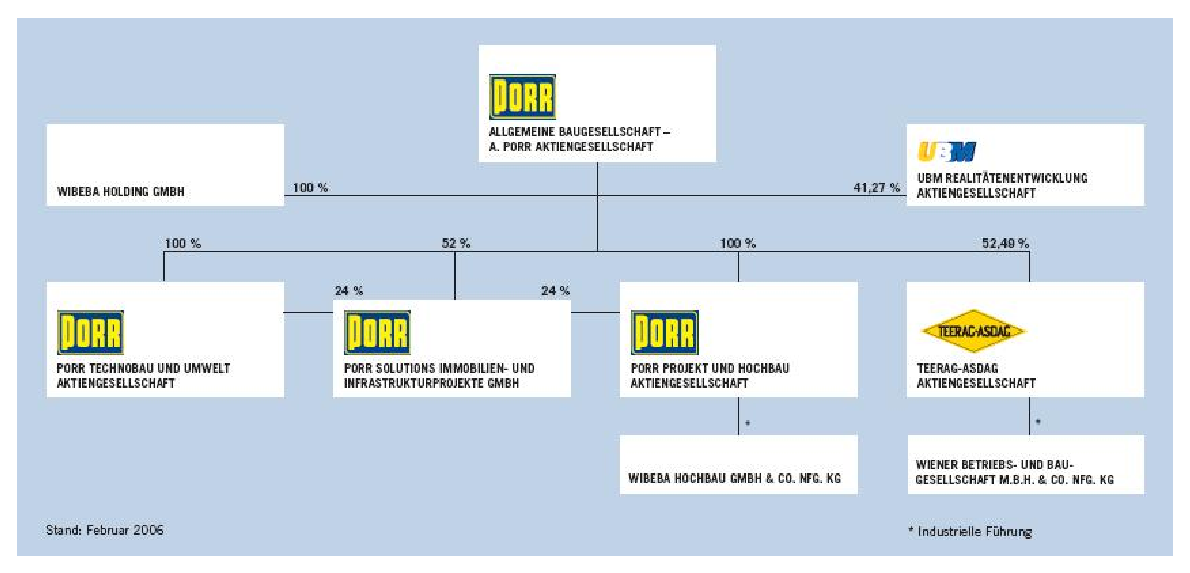
\includegraphics[width = \textwidth]{porr.eps}
	\caption{Porr Konzern�bersicht Quelle: \cite{porr}}
	\label{fig:porr}
\end{figure}